\section{A released-magnitude angular comparison in two depth bins}
A second observable can be studied without assigning the apparent CF4
tensor to a matter shear. We use the released Pantheon+ corrected
magnitudes and their total statistical-plus-systematic covariance,
retaining the original observation order and repeated supernova
observations. The primary sample contains 490 noncalibrator rows with
\(0.0233\le z_{\rm HD}\le0.15\); the lower-redshift sensitivity sample
contains 705 rows with \(0.01\le z_{\rm HD}\le0.15\). Both split at
\(z_{\rm HD}=0.06\), giving 342/148 and 557/148 low/high rows
respectively. The samples overlap.

Define the fixed dimensionless reference and residual

\[
 \mu_{\rm ref}=5\log_{10}\left[(1+z_{\rm HEL})
 \int_0^{z_{\rm HD}}\frac{dz}{\sqrt{0.3153(1+z)^3+0.6847}}\right],
 \qquad y=m_{b,\rm corr}-\mu_{\rm ref}.
\]

An additive magnitude intercept and one high-bin offset are profiled.
Neither is an independent absolute-Hubble-constant measurement. In each
bin, the angular response is \(d\cdot n+\sum_{A=1}^5q_A n^TE_An\), with
coefficients in magnitudes. The axes are the released RA/DEC Cartesian
chart; its physical reference-frame binding has not been established
here. The signed STF basis is

\[
 E_1=\operatorname{diag}(1,-1,0)/\sqrt2,\quad
 E_2=\operatorname{diag}(1,1,-2)/\sqrt6,\quad
 (E_3,E_4,E_5)=(e_xe_y^T+e_ye_x^T,
 e_xe_z^T+e_ze_x^T,e_ye_z^T+e_ze_y^T)/\sqrt2.
\]

Selection uses the marginal covariance \(C_s=P_s C_{\rm STAT+SYS}P_s^T\)
once, with the same original row indices on both axes. No separate
diagonal magnitude error, PV term, jitter or rescaling is added. The
complete released 1,701-row array contains 389 unordered pairs exceeding
the fixed symmetry tolerance, with maximum asymmetry
\(3.0\times10^{-8}\,\mathrm{mag}^2\). All affected pairs lie outside the
705-row selected union. Both consumed submatrices are exactly symmetric
as stored and positive definite. This validates the consumed submatrices
without certifying or repairing the unused full array.

After Cholesky whitening, both nuisance columns are projected out and
all 16 angular directions retain full rank. Let \(T_0\) and \(T_1\) be
the profiled nuisance-only and angular-model quadratic discrepancies.
Under the fixed-design Gaussian law with known selected covariance,
\(\Delta T=T_0-T_1\) has a conditional \(\chi^2_{16}\) reference. The
nominal 95-percent threshold is 26.2962.

\begin{table}[htbp]
\centering\small
\caption{Selected released-magnitude Gaussian comparisons; the total covariance is used once.}\label{tab:snfit}
\begin{tabular}{lllllll}
\toprule
Cohort & Low/high & $T_0$ & $T_{\rm dip}$ & $T_1$ & $\Delta T$ & $p$ \\
\midrule
Primary & 342/148 & 433.458517 & 426.408712 & 416.251929 & 17.206588 & 0.372352 \\
Lower redshift & 557/148 & 608.502006 & 598.873215 & 591.947917 & 16.554089 & 0.415003 \\
\bottomrule
\end{tabular}
\end{table}

\begin{table}[htbp]
\centering\small
\caption{All signed angular coordinates in mag, ordered $(d_x,d_y,d_z,q_1,\ldots,q_5)$. Full covariance matrices accompany the numerical supplement.}\label{tab:signed}
\begin{tabular}{lllll}
\toprule
Cohort & Coordinate & Low & High & High minus low \\
\midrule
Primary & 1 & +0.017576 & +0.002231 & -0.015344 \\
Primary & 2 & +0.030016 & +0.024261 & -0.005755 \\
Primary & 3 & +0.018480 & +0.058791 & +0.040311 \\
Primary & 4 & -0.024977 & +0.007323 & +0.032300 \\
Primary & 5 & -0.003468 & +0.102639 & +0.106107 \\
Primary & 6 & -0.028210 & -0.030533 & -0.002323 \\
Primary & 7 & +0.032482 & -0.036358 & -0.068840 \\
Primary & 8 & -0.036704 & -0.057764 & -0.021059 \\
Lower redshift & 1 & +0.016817 & +0.000080 & -0.016737 \\
Lower redshift & 2 & +0.031257 & +0.022736 & -0.008520 \\
Lower redshift & 3 & +0.025519 & +0.059176 & +0.033657 \\
Lower redshift & 4 & -0.006005 & +0.011789 & +0.017794 \\
Lower redshift & 5 & +0.006537 & +0.101451 & +0.094915 \\
Lower redshift & 6 & -0.019782 & -0.026867 & -0.007086 \\
Lower redshift & 7 & +0.023529 & -0.041688 & -0.065217 \\
Lower redshift & 8 & -0.027199 & -0.059823 & -0.032624 \\
\bottomrule
\end{tabular}
\end{table}

The primary improvement is 17.206588 with conditional upper-tail
probability 0.372352; lowering the minimum redshift gives 16.554089 and
0.415003. The primary comparison does not reject its isotropic two-level
nuisance model under this conditional law. Sixteen leave-one-survey
comparisons retain angular rank 16 and give improvements from 14.0415 to
18.9251. These correlated deletions describe sensitivity; they do not
calibrate an independent population null. All 50,616 low/high covariance
entries in the primary selected matrix are nonzero, and the complete
cross-bin covariance is retained.

\begin{figure}[htbp]
\centering
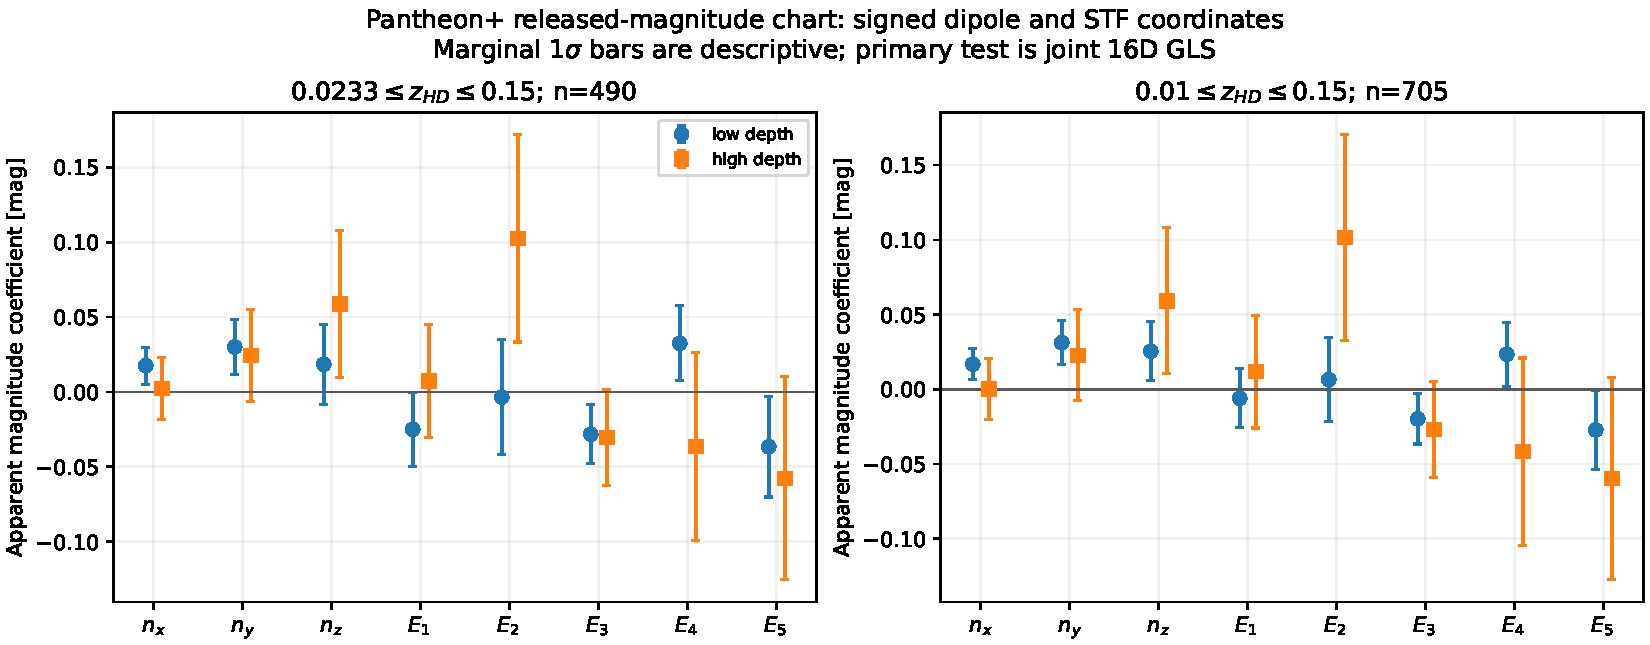
\includegraphics[width=0.95\linewidth]{r36_bridge/sn_signed.pdf}
\caption{Signed apparent-magnitude dipole and STF coordinates in the released Cartesian chart for the primary and overlapping lower-redshift sample. Error bars are marginal one-standard-deviation displays. Inference uses the full joint covariance and the prespecified 16-coordinate comparison; individual bars are not simultaneous acceptance intervals or separate binwise tests.}
\end{figure}

The chart \(d_{L*}=d_L/(1+z_{\rm HEL})^2\) subtracts
\(10\log_{10}(1+z_{\rm HEL})\) from both observed magnitude and
reference mean at fixed released redshifts. The residual and its fitted
coefficients are therefore invariant; the retained real-data coefficient
change is below \(10^{-14}\) mag. Subtracting from only one side changes
the residual and fails this consistency test. A physical observer boost
also changes photon redshift, direction, distance response and
potentially selection and uncertainty, so chart invariance is not a
boosted-observer fit. The released \(z_{\rm HD}\) includes its
peculiar-velocity correction; \(z_{\rm CMB}\) is retained and is not
substituted for the photon-redshift factor.

These magnitude tensors are a separate released-observable estimand.
They do not establish nominal light-curve-training parity, a
material-frame shear, acceleration, or a physical observer velocity. The
supernova and CF4 comparisons have neither a supplied common response
nor a measured shared-PV cross-covariance, so their statistics are not
added and their probabilities are not multiplied. Their useful common
output is a signed, covariance-aware description of apparent angular
structure with explicit depth support.
